As a cross-check of the main analysis, we have also performed the shape-based 
procedure using two different distributions: $\mll$ and the BDT classifier 
used with the $\sqrt{s}=~7~\TeV$ energy in 2011. The expected and observed upper 
limits are reported in Tables~\ref{tab:mvabase_mll_0j} to~\ref{tab:mvabase_bdt2011_nj}, and 
in Figures~\ref{fig:uls_mll} and~\ref{fig:uls_bdt2011}.

%%%%%%%%%%%%%%%%%%%%%%%%%%%%%%
\begin{table}[hbp!]
\begin{center}
\begin{tabular}{c c c c c}
\hline
\vspace{-3mm} && \\
 Higgs Mass & Observed  & Median expected & Expected range for 68\% & Expected range for 95\%   \\
\vspace{-3mm} && \\
\hline
110 & 12.12 & 7.68 & [5.53, 10.68] & [4.12, 14.32] \\
115 & 4.88 & 3.65 & [2.63, 5.08] & [1.96, 6.82] \\
120 & 3.90 & 2.22 & [1.60, 3.09] & [1.19, 4.14] \\
125 & 2.23 & 1.33 & [0.96, 1.85] & [0.71, 2.48] \\
130 & 1.68 & 0.97 & [0.70, 1.35] & [0.52, 1.81] \\
135 & 1.19 & 0.71 & [0.51, 0.98] & [0.38, 1.32] \\
140 & 0.99 & 0.62 & [0.44, 0.86] & [0.33, 1.15] \\
145 & 0.92 & 0.52 & [0.37, 0.72] & [0.28, 0.96] \\
150 & 0.72 & 0.46 & [0.33, 0.64] & [0.25, 0.85] \\
155 & 0.56 & 0.36 & [0.26, 0.50] & [0.19, 0.67] \\
160 & 0.49 & 0.33 & [0.24, 0.46] & [0.18, 0.61] \\
170 & 0.58 & 0.38 & [0.28, 0.53] & [0.21, 0.71] \\
180 & 0.81 & 0.56 & [0.40, 0.78] & [0.30, 1.04] \\
190 & 0.99 & 0.84 & [0.61, 1.18] & [0.45, 1.58] \\
200 & 1.48 & 1.11 & [0.80, 1.54] & [0.59, 2.07] \\
250 & 1.30 & 1.40 & [1.01, 1.95] & [0.75, 2.62] \\
300 & 1.27 & 1.65 & [1.19, 2.30] & [0.89, 3.08] \\
350 & 1.31 & 1.55 & [1.12, 2.16] & [0.83, 2.90] \\
400 & 1.52 & 1.66 & [1.20, 2.31] & [0.89, 3.10] \\
450 & 1.89 & 2.20 & [1.59, 3.06] & [1.18, 4.10] \\
500 & 3.47 & 3.38 & [2.44, 4.70] & [1.81, 6.31] \\
550 & 4.87 & 4.90 & [3.53, 6.82] & [2.63, 9.15] \\
600 & 7.32 & 7.23 & [5.21, 10.07] & [3.88, 13.49] \\
\hline
\end{tabular}
\caption{Expected and observed upper limits in the 0-jet bin for SM Higgs using the
  {\bf shape-based} $\mll$ analysis with 3.5$\ifb$ of data.}
\label{tab:mvabase_mll_0j}
\end{center}
\end{table}
%%%%%%%%%%%%%%%%%%%%%%%%%%%%%%
%%%%%%%%%%%%%%%%%%%%%%%%%%%%%%
\begin{table}[hbp!]
\begin{center}
\begin{tabular}{c c c c c}
\hline
\vspace{-3mm} && \\
 Higgs Mass & Observed  & Median expected & Expected range for 68\% & Expected range for 95\%   \\
\vspace{-3mm} && \\
\hline
110 & 8.23 & 9.98 & [7.19, 13.89] & [5.36, 18.62] \\
115 & 8.35 & 6.25 & [4.50, 8.70] & [3.35, 11.66] \\
120 & 4.38 & 3.81 & [2.74, 5.30] & [2.04, 7.10] \\
125 & 3.54 & 2.19 & [1.58, 3.05] & [1.18, 4.09] \\
130 & 2.45 & 1.50 & [1.08, 2.09] & [0.81, 2.80] \\
135 & 1.84 & 1.15 & [0.83, 1.60] & [0.62, 2.14] \\
140 & 1.53 & 1.04 & [0.75, 1.45] & [0.56, 1.94] \\
145 & 1.27 & 0.84 & [0.60, 1.16] & [0.45, 1.56] \\
150 & 1.16 & 0.74 & [0.53, 1.03] & [0.40, 1.38] \\
155 & 1.02 & 0.57 & [0.41, 0.79] & [0.30, 1.06] \\
160 & 0.91 & 0.48 & [0.34, 0.66] & [0.26, 0.89] \\
170 & 0.98 & 0.54 & [0.39, 0.76] & [0.29, 1.02] \\
180 & 0.98 & 0.71 & [0.51, 0.99] & [0.38, 1.32] \\
190 & 0.97 & 1.08 & [0.77, 1.50] & [0.58, 2.01] \\
200 & 1.07 & 1.41 & [1.02, 1.97] & [0.76, 2.64] \\
250 & 1.12 & 2.01 & [1.45, 2.79] & [1.08, 3.74] \\
300 & 1.06 & 2.13 & [1.54, 2.97] & [1.14, 3.98] \\
350 & 1.70 & 1.75 & [1.26, 2.44] & [0.94, 3.27] \\
400 & 2.31 & 2.12 & [1.53, 2.96] & [1.14, 3.96] \\
450 & 3.53 & 2.97 & [2.14, 4.13] & [1.59, 5.53] \\
500 & 6.17 & 4.27 & [3.08, 5.94] & [2.29, 7.97] \\
550 & 10.99 & 5.81 & [4.19, 8.09] & [3.12, 10.84] \\
600 & 11.85 & 8.13 & [5.86, 11.32] & [4.36, 15.17] \\
\hline
\end{tabular}
\caption{Expected and observed upper limits in the 1-jet bin for SM Higgs using the
  {\bf shape-based} $\mll$ analysis with 3.5$\ifb$ of data.}
\label{tab:mvabase_mll_1j}
\end{center}
\end{table}
%%%%%%%%%%%%%%%%%%%%%%%%%%%%%%
%%%%%%%%%%%%%%%%%%%%%%%%%%%%%%
\begin{table}[hbp!]
\begin{center}
\begin{tabular}{c c c c c}
\hline
\vspace{-3mm} && \\
 Higgs Mass & Observed  & Median expected & Expected range for 68\% & Expected range for 95\%   \\
\vspace{-3mm} && \\
\hline
110 & 8.11 & 5.85 & [4.21, 8.14] & [3.14, 10.91] \\
115 & 4.39 & 3.06 & [2.20, 4.25] & [1.64, 5.70] \\
120 & 3.49 & 1.84 & [1.33, 2.56] & [0.99, 3.44] \\
125 & 1.99 & 1.11 & [0.80, 1.54] & [0.59, 2.07] \\
130 & 1.51 & 0.79 & [0.57, 1.10] & [0.42, 1.47] \\
135 & 1.10 & 0.59 & [0.43, 0.82] & [0.32, 1.10] \\
140 & 0.91 & 0.52 & [0.37, 0.72] & [0.28, 0.96] \\
145 & 0.83 & 0.43 & [0.31, 0.59] & [0.23, 0.79] \\
150 & 0.67 & 0.38 & [0.27, 0.53] & [0.20, 0.71] \\
155 & 0.64 & 0.32 & [0.23, 0.44] & [0.17, 0.60] \\
160 & 0.52 & 0.28 & [0.20, 0.38] & [0.15, 0.52] \\
170 & 0.60 & 0.32 & [0.23, 0.44] & [0.17, 0.59] \\
180 & 0.59 & 0.43 & [0.31, 0.60] & [0.23, 0.81] \\
190 & 0.70 & 0.65 & [0.47, 0.90] & [0.35, 1.21] \\
200 & 1.08 & 0.84 & [0.60, 1.16] & [0.45, 1.56] \\
250 & 0.65 & 1.08 & [0.78, 1.50] & [0.58, 2.01] \\
300 & 0.56 & 1.15 & [0.83, 1.61] & [0.62, 2.15] \\
350 & 0.83 & 1.01 & [0.73, 1.40] & [0.54, 1.88] \\
400 & 1.11 & 1.15 & [0.83, 1.60] & [0.62, 2.15] \\
450 & 1.47 & 1.57 & [1.13, 2.19] & [0.85, 2.94] \\
500 & 2.82 & 2.41 & [1.74, 3.35] & [1.29, 4.50] \\
550 & 4.80 & 3.25 & [2.34, 4.52] & [1.74, 6.06] \\
600 & 6.92 & 4.61 & [3.32, 6.42] & [2.48, 8.61] \\
\hline
\end{tabular}
\caption{Expected and observed upper limits in the 0/1-jet bins for SM Higgs using the
  {\bf shape-based} $\mll$ analysis with 3.5$\ifb$ of data.}
\label{tab:mvabase_mll_nj}
\end{center}
\end{table}
%%%%%%%%%%%%%%%%%%%%%%%%%%%%%%

%%%%%%%%%%%%%%%%%%%%%%%%%%%%%%
\begin{table}[hbp!]
\begin{center}
\begin{tabular}{c c c c c}
\hline
\vspace{-3mm} && \\
 Higgs Mass & Observed  & Median expected & Expected range for 68\% & Expected range for 95\%   \\
\vspace{-3mm} && \\
\hline
110 & 11.54 & 6.24 & [4.49, 8.68] & [3.35, 11.64] \\
115 & 6.03 & 3.34 & [2.41, 4.65] & [1.79, 6.23] \\
120 & 2.99 & 3.10 & [2.23, 4.31] & [1.66, 5.77] \\
130 & 2.04 & 0.94 & [0.68, 1.30] & [0.50, 1.75] \\
135 & 1.44 & 0.77 & [0.55, 1.07] & [0.41, 1.43] \\
140 & 1.04 & 0.61 & [0.44, 0.85] & [0.33, 1.14] \\
150 & 0.86 & 0.40 & [0.29, 0.56] & [0.22, 0.75] \\
160 & 0.50 & 0.25 & [0.18, 0.35] & [0.13, 0.47] \\
170 & 0.46 & 0.27 & [0.19, 0.37] & [0.14, 0.50] \\
180 & 0.50 & 0.34 & [0.24, 0.47] & [0.18, 0.63] \\
190 & 0.87 & 0.50 & [0.36, 0.70] & [0.27, 0.94] \\
200 & 1.02 & 0.62 & [0.45, 0.87] & [0.34, 1.16] \\
250 & 1.10 & 1.07 & [0.77, 1.49] & [0.57, 1.99] \\
300 & 1.35 & 1.49 & [1.07, 2.07] & [0.80, 2.77] \\
350 & 1.15 & 1.30 & [0.94, 1.81] & [0.70, 2.43] \\
400 & 1.73 & 1.39 & [1.00, 1.94] & [0.75, 2.59] \\
450 & 1.62 & 1.75 & [1.26, 2.43] & [0.94, 3.26] \\
500 & 4.33 & 3.42 & [2.46, 4.76] & [1.84, 6.38] \\
550 & 4.51 & 3.52 & [2.54, 4.90] & [1.89, 6.57] \\
600 & 7.53 & 7.36 & [5.30, 10.24] & [3.95, 13.72] \\
\hline
\end{tabular}
\caption{Expected and observed upper limits in the 0-jet bin for SM Higgs using the
  {\bf shape-based} 2011 BDT analysis with 3.5$\ifb$ of data.}
\label{tab:mvabase_bdt2011_0j}
\end{center}
\end{table}
%%%%%%%%%%%%%%%%%%%%%%%%%%%%%%
%%%%%%%%%%%%%%%%%%%%%%%%%%%%%%
\begin{table}[hbp!]
\begin{center}
\begin{tabular}{c c c c c}
\hline
\vspace{-3mm} && \\
 Higgs Mass & Observed  & Median expected & Expected range for 68\% & Expected range for 95\%   \\
\vspace{-3mm} && \\
\hline
110 & 10.23 & 11.41 & [8.22, 15.87] & [6.12, 21.28] \\
115 & 5.54 & 5.88 & [4.23, 8.18] & [3.15, 10.96] \\
120 & 4.73 & 4.68 & [3.37, 6.52] & [2.51, 8.73] \\
130 & 2.13 & 1.41 & [1.02, 1.97] & [0.76, 2.64] \\
135 & 1.62 & 1.09 & [0.79, 1.52] & [0.59, 2.04] \\
140 & 1.14 & 0.85 & [0.61, 1.18] & [0.45, 1.58] \\
150 & 0.81 & 0.62 & [0.44, 0.86] & [0.33, 1.15] \\
160 & 0.65 & 0.36 & [0.26, 0.51] & [0.19, 0.68] \\
170 & 0.74 & 0.41 & [0.29, 0.57] & [0.22, 0.76] \\
180 & 1.00 & 0.52 & [0.37, 0.72] & [0.28, 0.97] \\
190 & 1.41 & 0.80 & [0.57, 1.11] & [0.43, 1.49] \\
200 & 1.99 & 1.09 & [0.78, 1.51] & [0.58, 2.03] \\
250 & 1.48 & 1.70 & [1.22, 2.36] & [0.91, 3.16] \\
300 & 1.27 & 1.89 & [1.36, 2.63] & [1.01, 3.52] \\
350 & 1.10 & 1.58 & [1.14, 2.19] & [0.85, 2.94] \\
400 & 1.23 & 1.88 & [1.35, 2.61] & [1.01, 3.50] \\
450 & 1.79 & 2.55 & [1.84, 3.55] & [1.37, 4.76] \\
500 & 4.08 & 3.57 & [2.57, 4.97] & [1.92, 6.66] \\
550 & 4.52 & 4.60 & [3.32, 6.40] & [2.47, 8.58] \\
600 & 6.46 & 7.07 & [5.09, 9.83] & [3.79, 13.18] \\
\hline
\end{tabular}
\caption{Expected and observed upper limits in the 1-jet bin for SM Higgs using the
  {\bf shape-based} 2011 BDT analysis with 3.5$\ifb$ of data.}
\label{tab:mvabase_bdt2011_1j}
\end{center}
\end{table}
%%%%%%%%%%%%%%%%%%%%%%%%%%%%%%
%%%%%%%%%%%%%%%%%%%%%%%%%%%%%%
\begin{table}[hbp!]
\begin{center}
\begin{tabular}{c c c c c}
\hline
\vspace{-3mm} && \\
 Higgs Mass & Observed  & Median expected & Expected range for 68\% & Expected range for 95\%   \\
\vspace{-3mm} && \\
\hline
110 & 8.18 & 5.26 & [3.79, 7.31] & [2.82, 9.80] \\
115 & 4.82 & 2.75 & [1.98, 3.83] & [1.48, 5.13] \\
120 & 2.71 & 2.66 & [1.91, 3.70] & [1.43, 4.95] \\
130 & 1.36 & 0.75 & [0.54, 1.05] & [0.40, 1.40] \\
135 & 1.11 & 0.62 & [0.45, 0.86] & [0.33, 1.15] \\
140 & 0.92 & 0.48 & [0.35, 0.67] & [0.26, 0.90] \\
150 & 0.63 & 0.34 & [0.24, 0.47] & [0.18, 0.63] \\
160 & 0.41 & 0.22 & [0.16, 0.30] & [0.12, 0.41] \\
170 & 0.44 & 0.24 & [0.17, 0.33] & [0.13, 0.44] \\
180 & 0.51 & 0.29 & [0.21, 0.40] & [0.15, 0.54] \\
190 & 0.74 & 0.42 & [0.31, 0.59] & [0.23, 0.79] \\
200 & 0.99 & 0.54 & [0.39, 0.75] & [0.29, 1.01] \\
250 & 0.73 & 0.87 & [0.63, 1.21] & [0.47, 1.63] \\
300 & 1.13 & 1.04 & [0.75, 1.44] & [0.56, 1.93] \\
350 & 0.49 & 0.86 & [0.62, 1.19] & [0.46, 1.60] \\
400 & 0.96 & 1.03 & [0.74, 1.44] & [0.55, 1.92] \\
450 & 1.12 & 1.32 & [0.95, 1.84] & [0.71, 2.46] \\
500 & 2.05 & 2.30 & [1.66, 3.20] & [1.23, 4.29] \\
550 & 3.04 & 2.51 & [1.81, 3.49] & [1.35, 4.68] \\
600 & 5.80 & 4.66 & [3.36, 6.48] & [2.50, 8.69] \\
\hline
\end{tabular}
\caption{Expected and observed upper limits in the 0/1-jet bins for SM Higgs using the
  {\bf shape-based} 2011 BDT analysis with 3.5$\ifb$ of data.}
\label{tab:mvabase_bdt2011_nj}
\end{center}
\end{table}

%%%%%%%%%%%%%%%%%%%%%%%%%%%%%%
\begin{figure}[!hbtp]
\centering
\subfigure[shape-based $\mll$ 0-jet bin]{
\centering
\label{subfig:sm_shape_mll_0j}
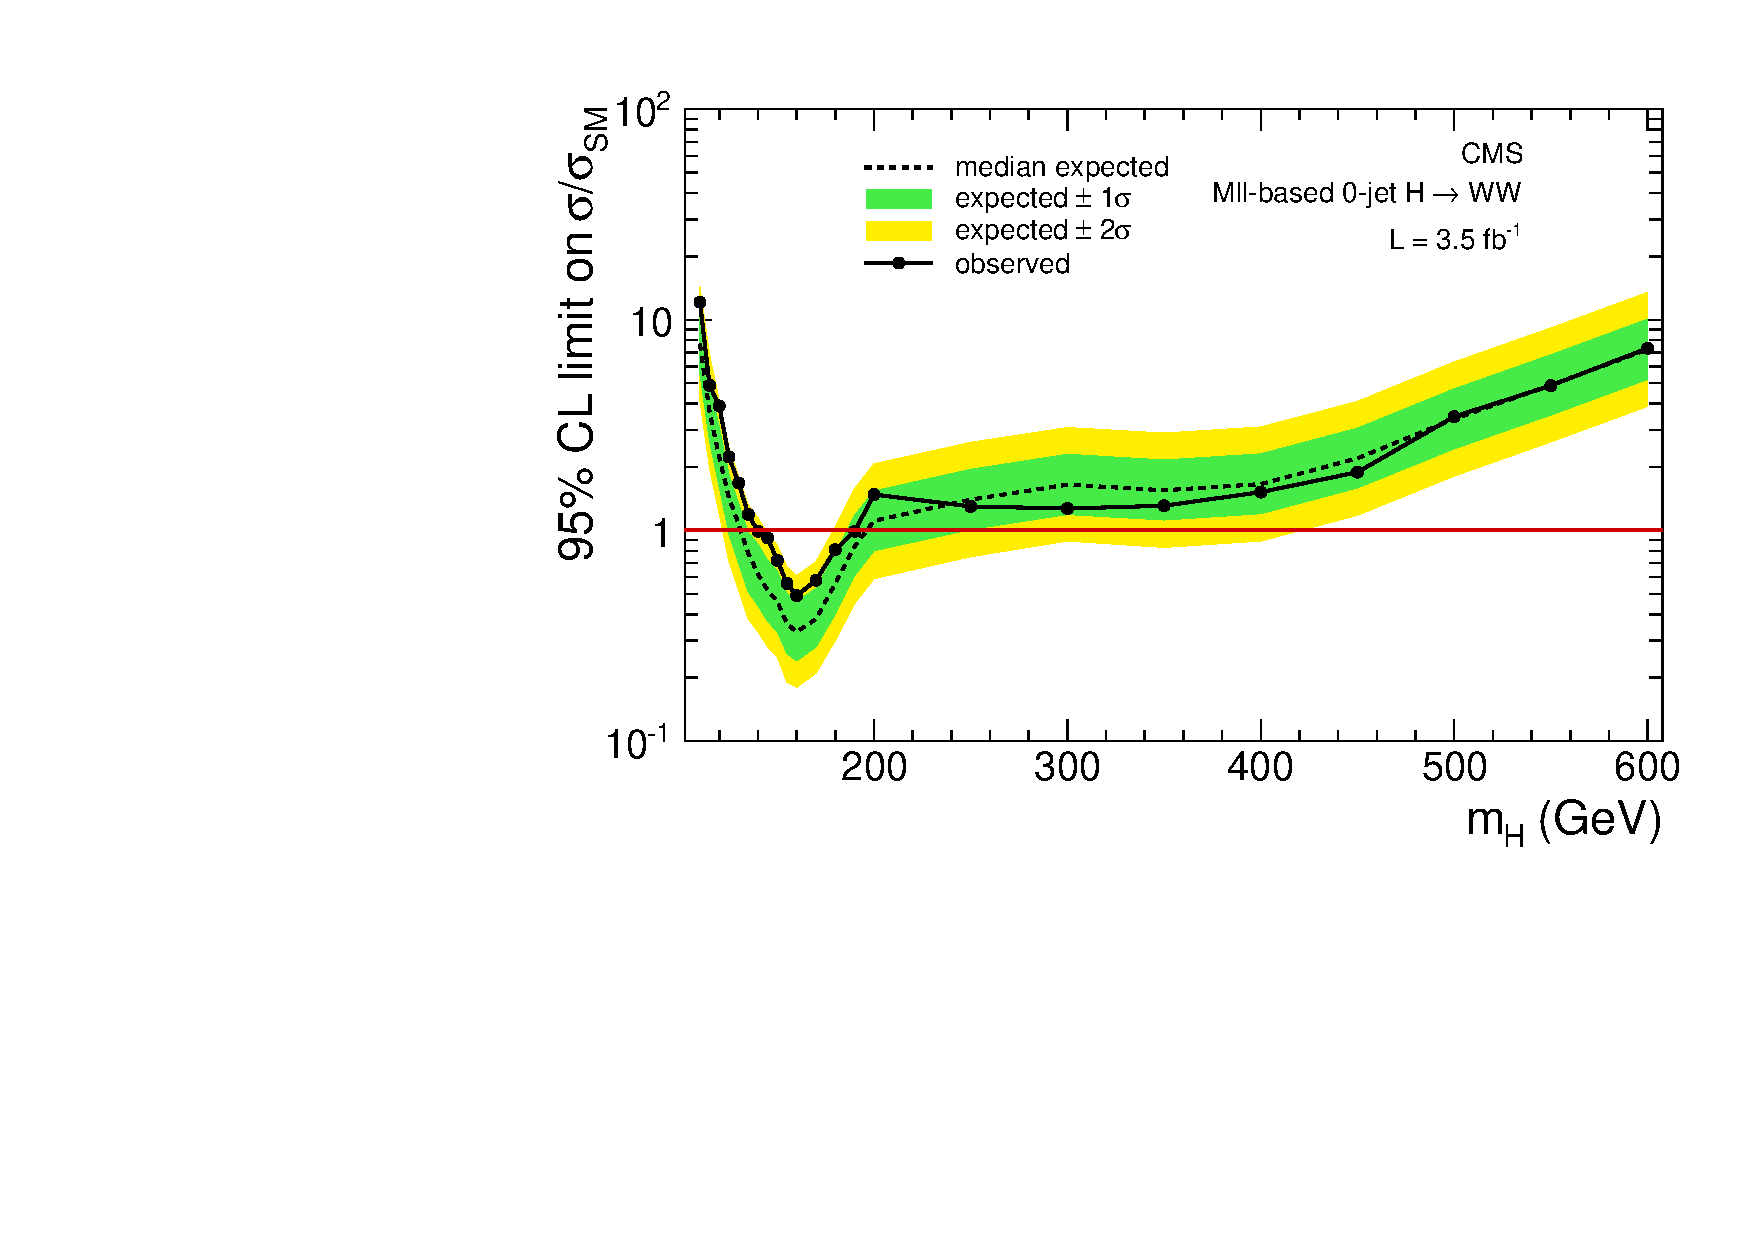
\includegraphics[width=.45\textwidth]{figures/limits_0j_Mll_shape_extended_8TeV.pdf}
}
\subfigure[shape-based zoomed $\mll$ 0-jet bin]{
\centering
\label{subfig:sm_shape_zoom_mll_0j}
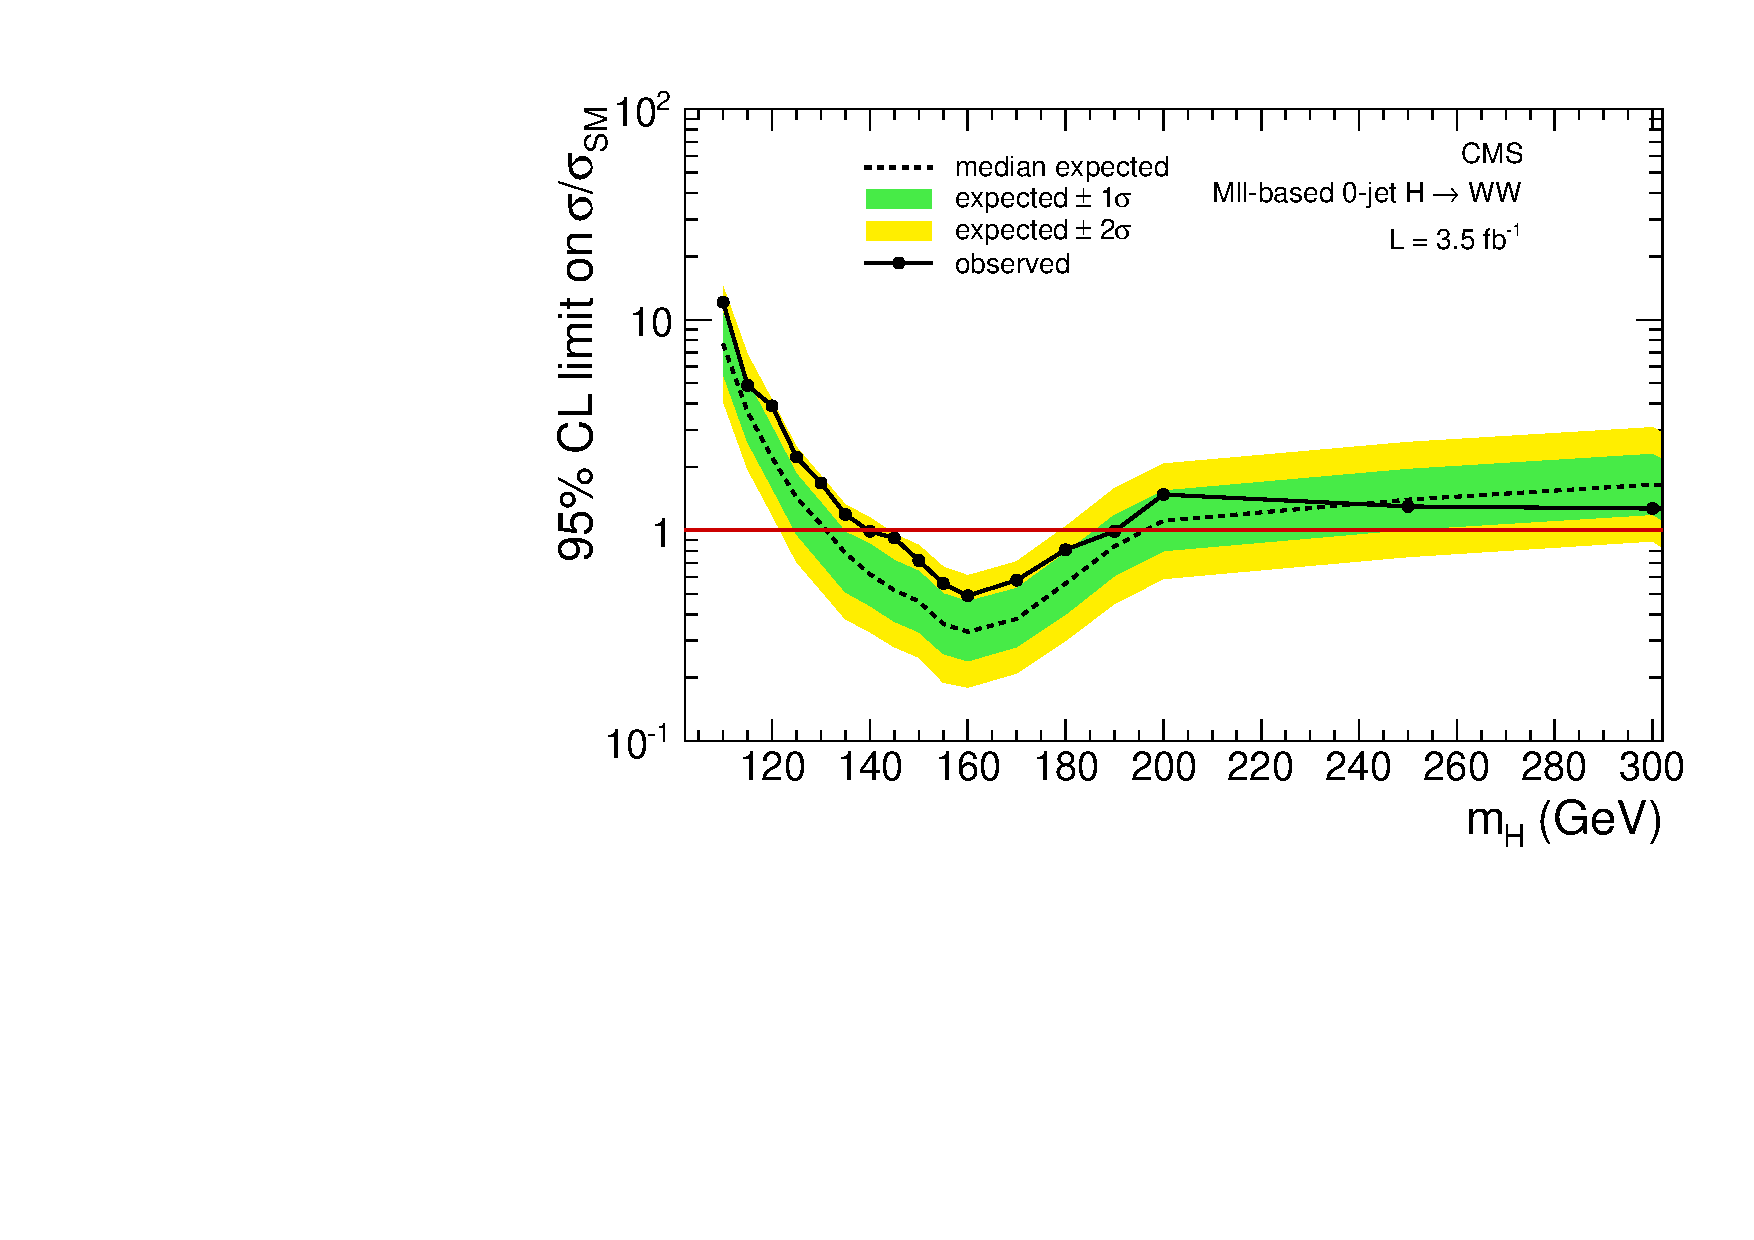
\includegraphics[width=.45\textwidth]{figures/limits_0j_Mll_shape_8TeV.pdf}
}
\centering
\subfigure[shape-based $\mll$ 1-jet bin]{
\centering
\label{subfig:sm_shape_mll_1j}
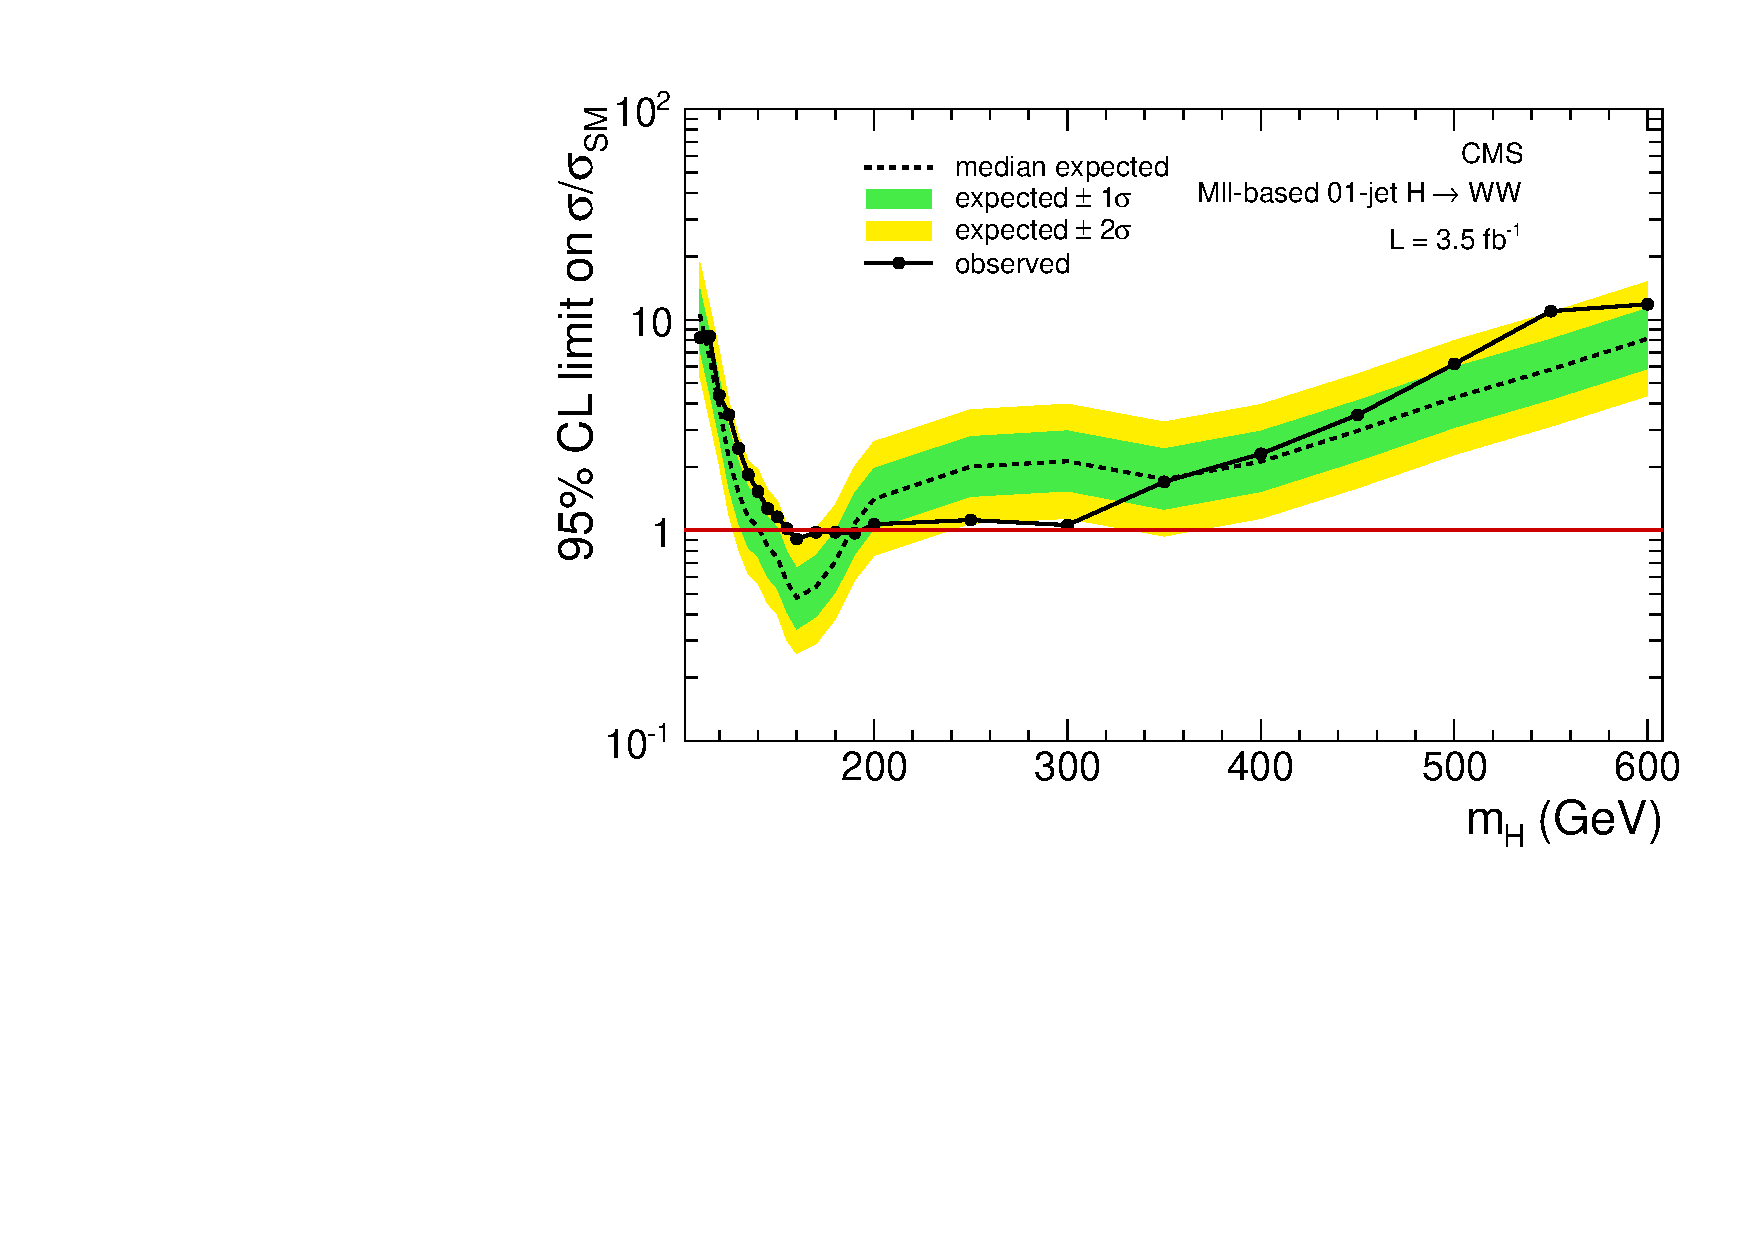
\includegraphics[width=.45\textwidth]{figures/limits_1j_Mll_shape_extended_8TeV.pdf}
}
\subfigure[shape-based zoomed $\mll$ 1-jet bin]{
\centering
\label{subfig:sm_shape_zoom_mll_1j}
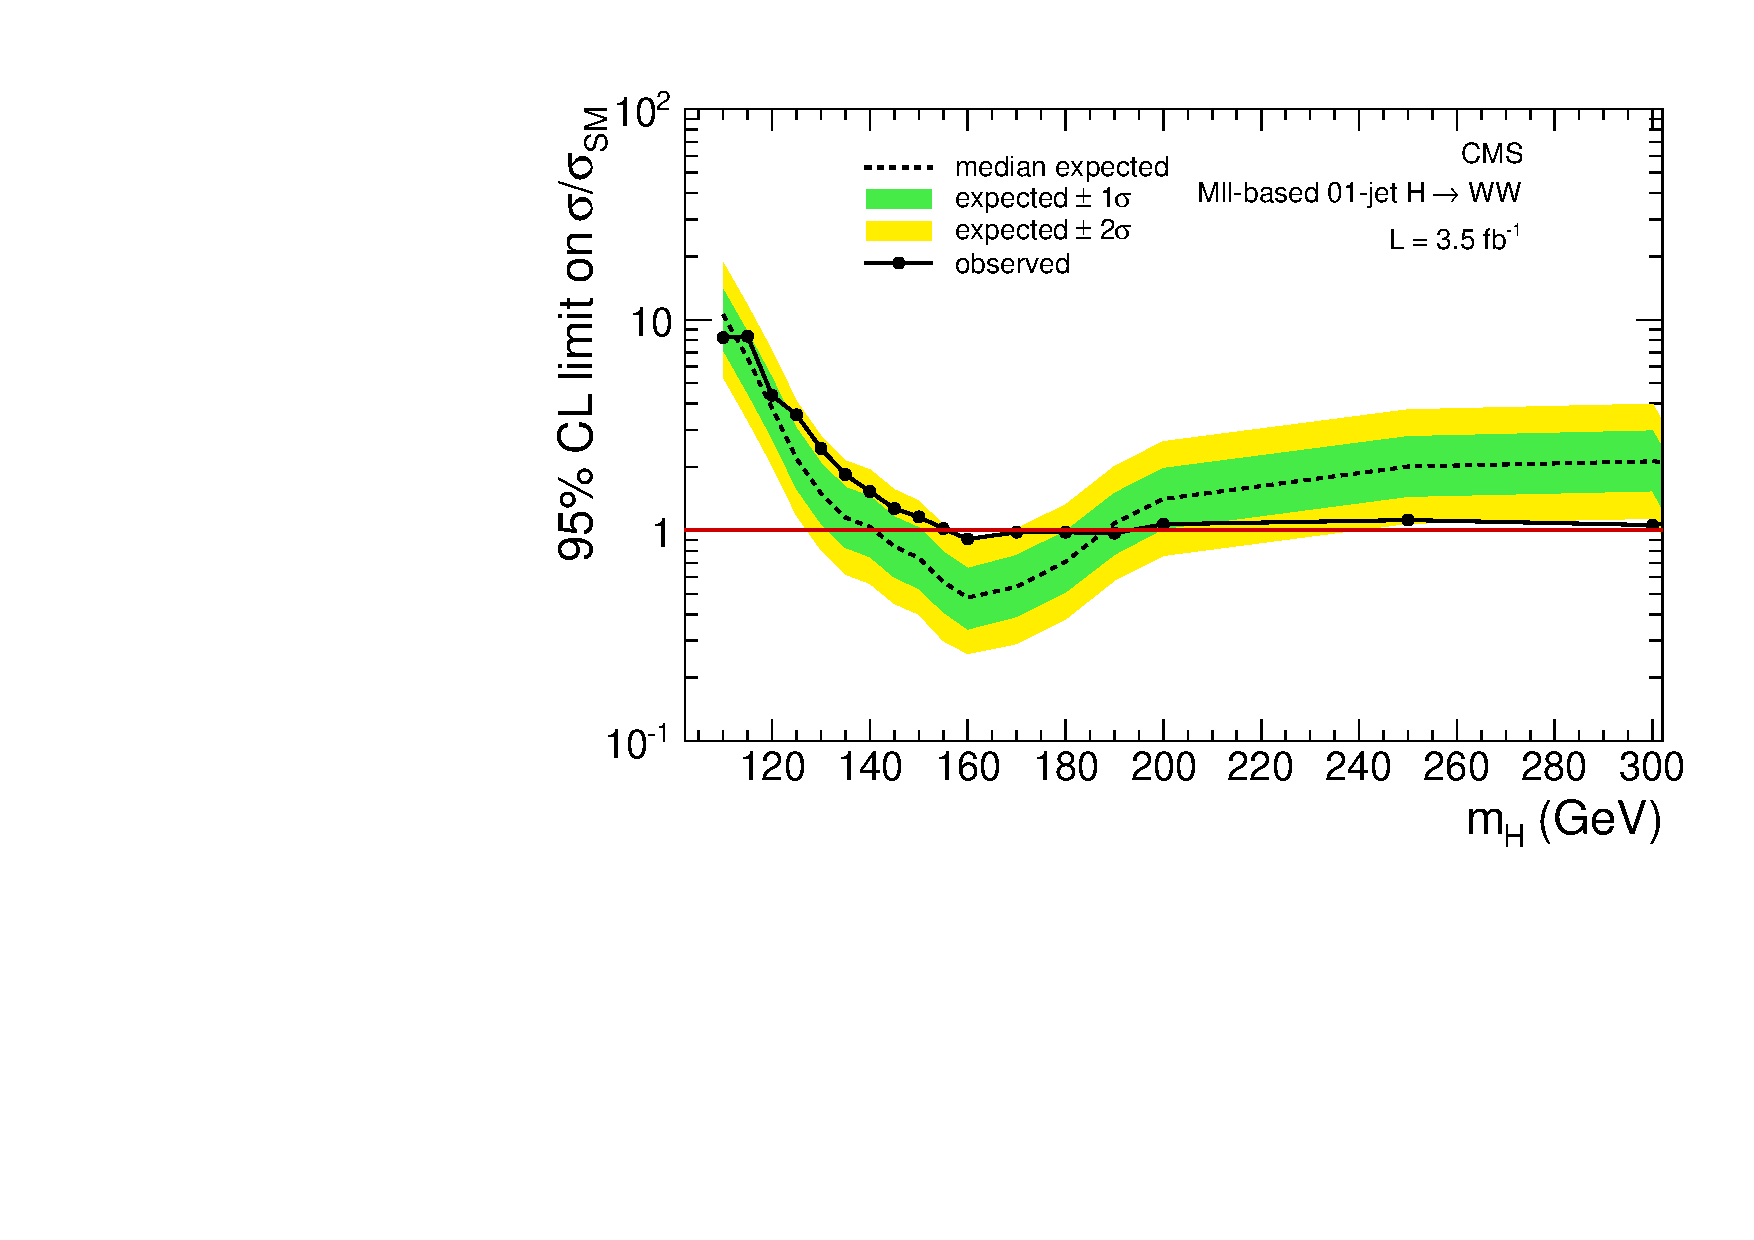
\includegraphics[width=.45\textwidth]{figures/limits_1j_Mll_shape_8TeV.pdf}
}
\centering
\subfigure[shape-based $\mll$ 0/1-jet bins]{
\centering
\label{subfig:sm_shape_mll_nj}
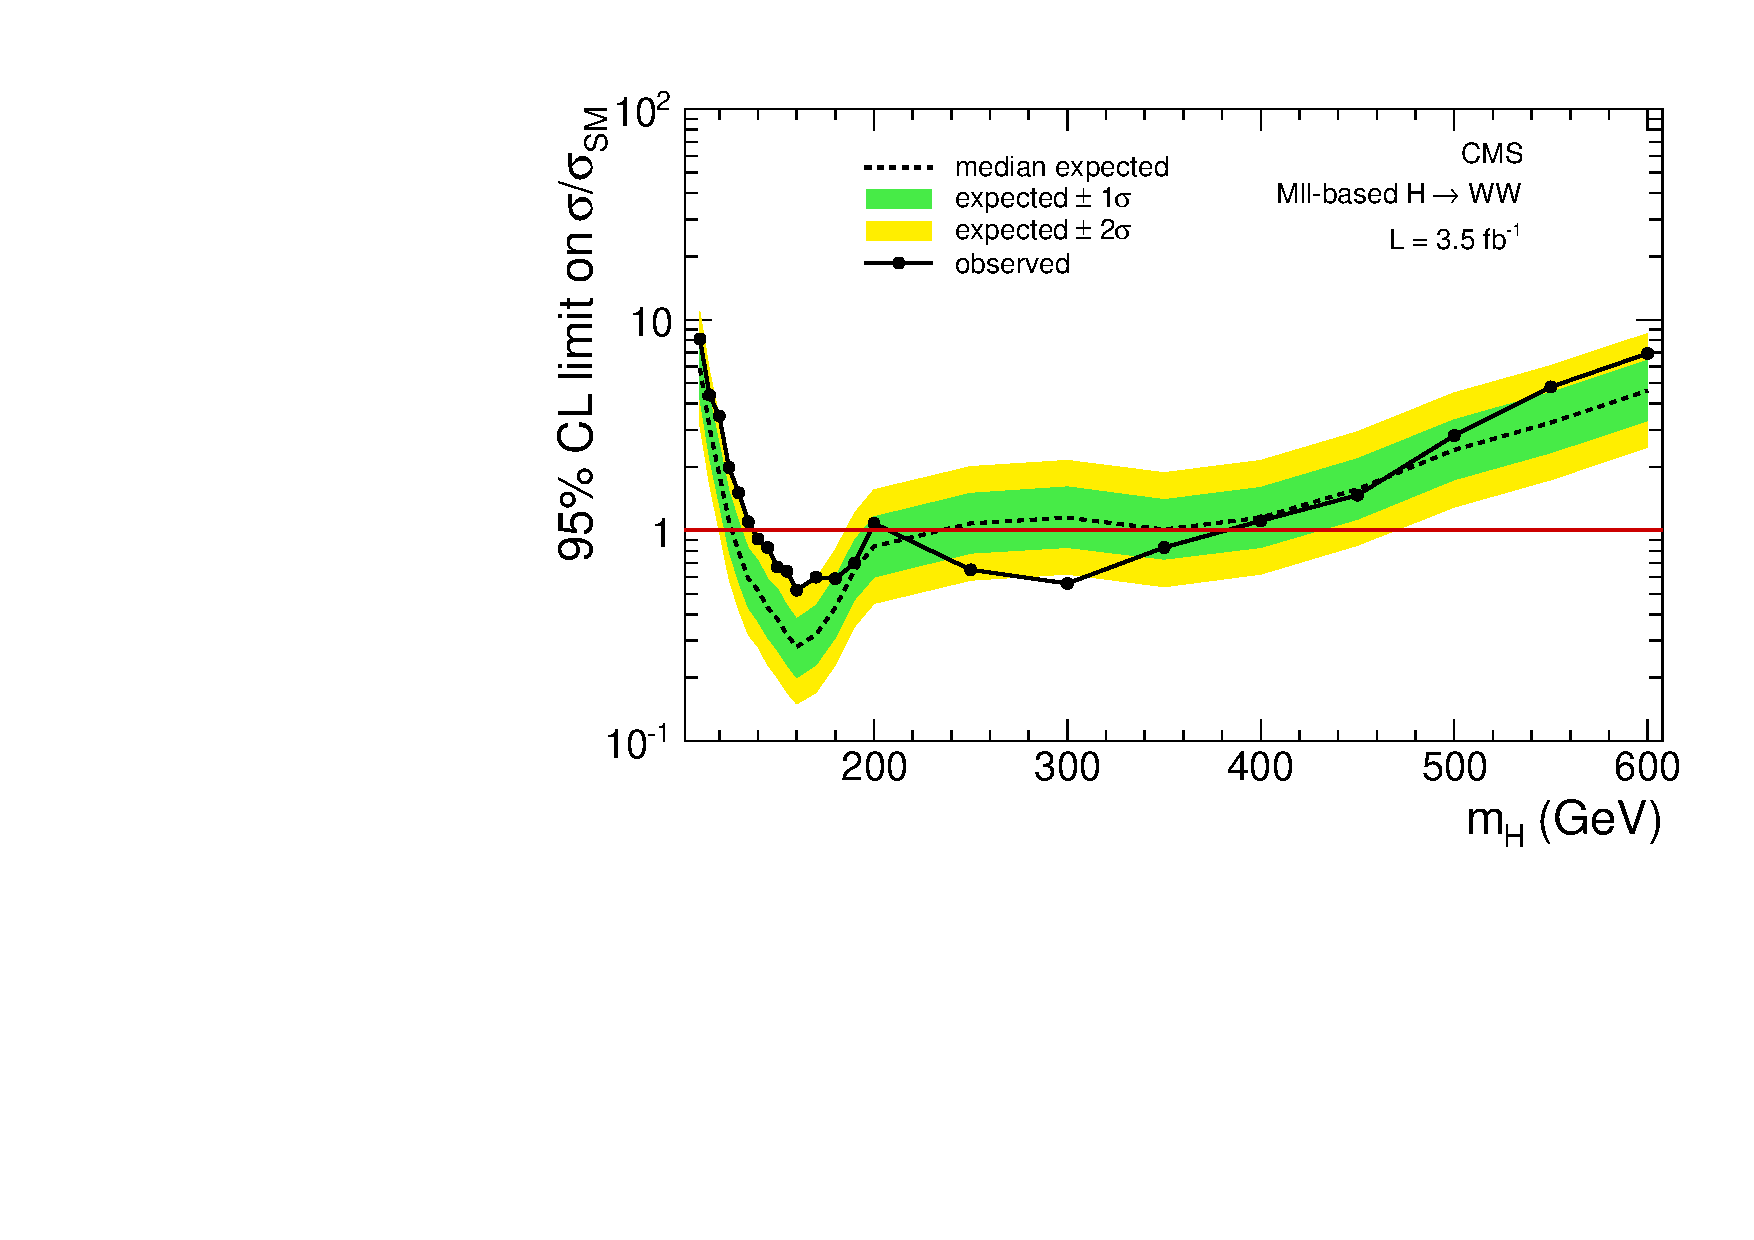
\includegraphics[width=.45\textwidth]{figures/limits_nj_Mll_shape_extended_8TeV.pdf}
}
\subfigure[shape-based zoomed $\mll$ 0/1-jet bins]{
\centering
\label{subfig:sm_shape_zoom_mll_nj}
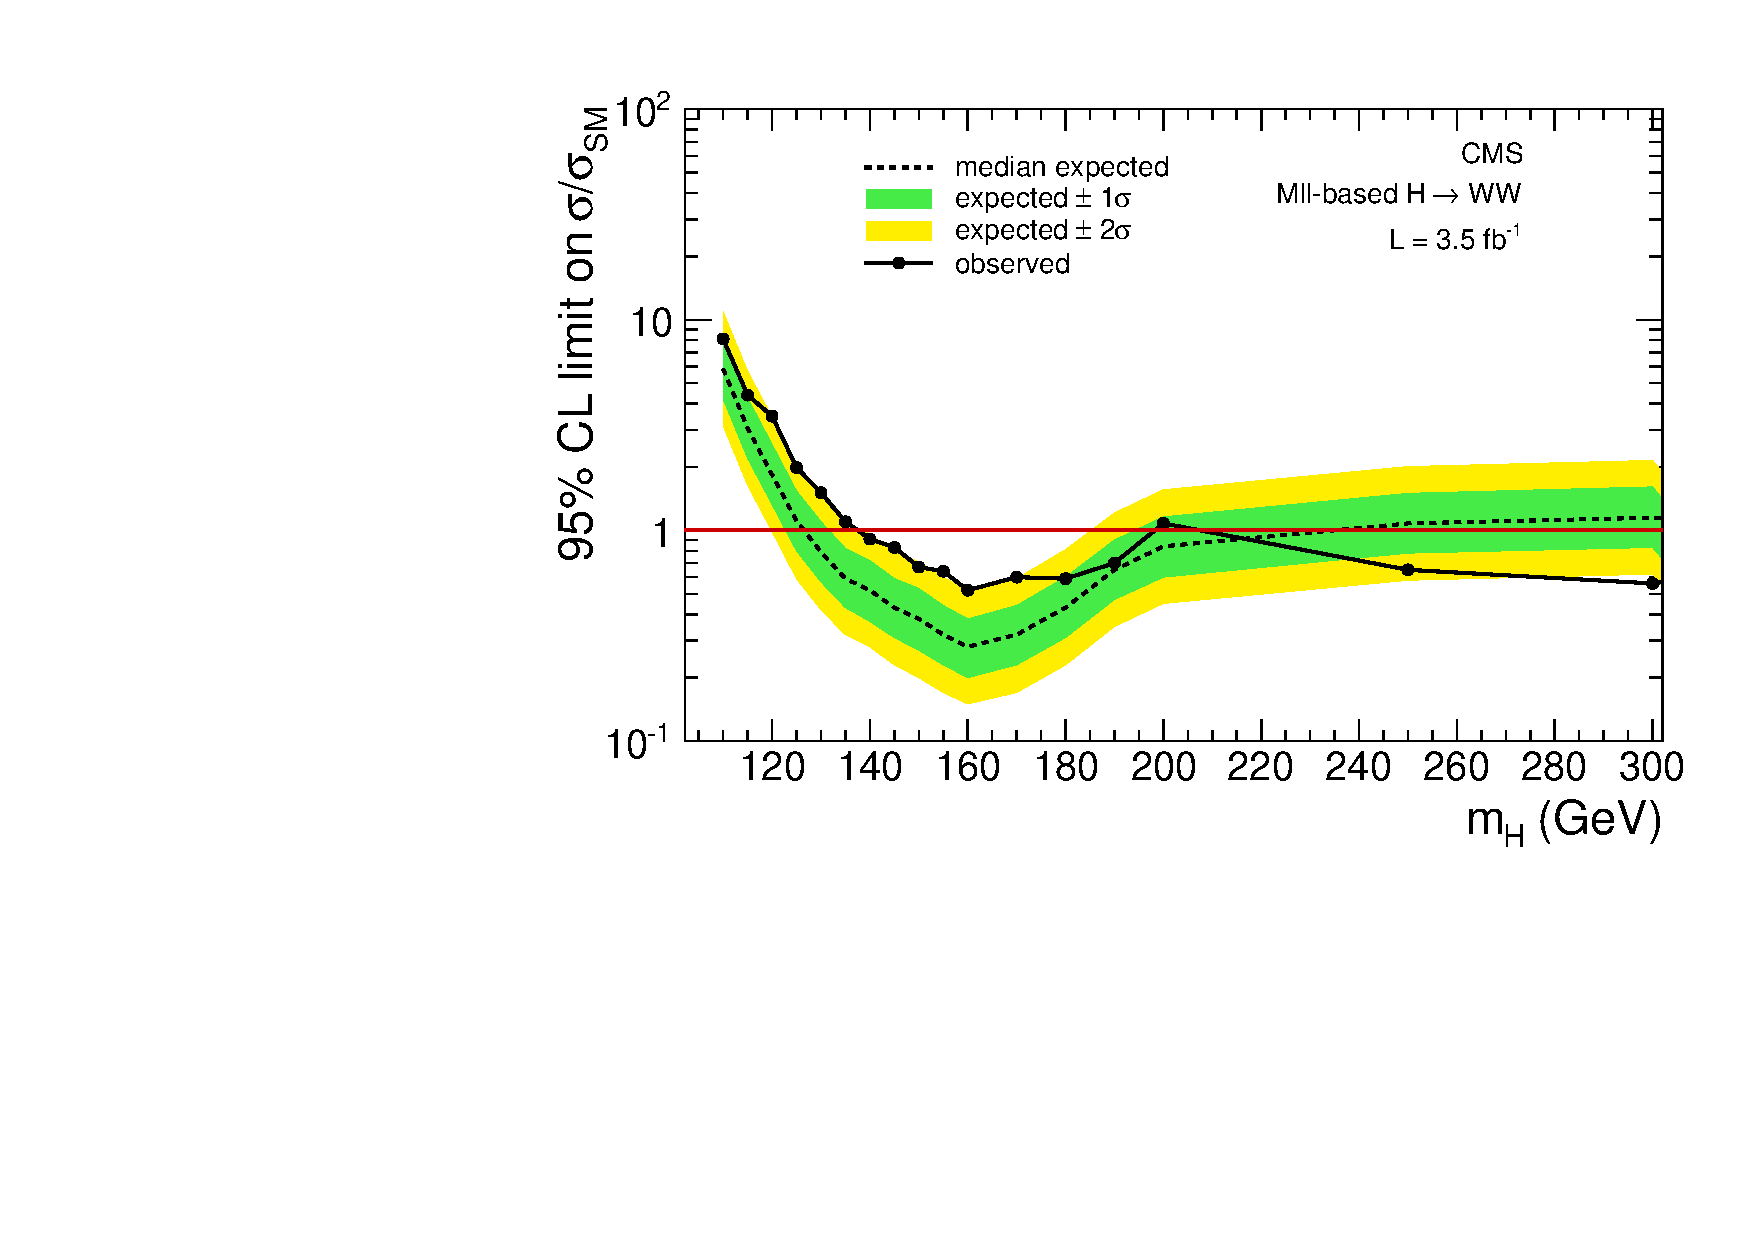
\includegraphics[width=.45\textwidth]{figures/limits_nj_Mll_shape_8TeV.pdf}
}
\caption{Expected and observed upper limits for SM Higgs using the
  {\bf shape-based} $\mll$ analysis with 3.5 $\ifb$ of data.}
\label{fig:uls_mll}
\end{figure}

%%%%%%%%%%%%%%%%%%%%%%%%%%%%%%
\begin{figure}[!hbtp]
\centering
\subfigure[shape-based 2011 BDT 0-jet bin]{
\centering
\label{subfig:sm_shape_BDT2011_0j}
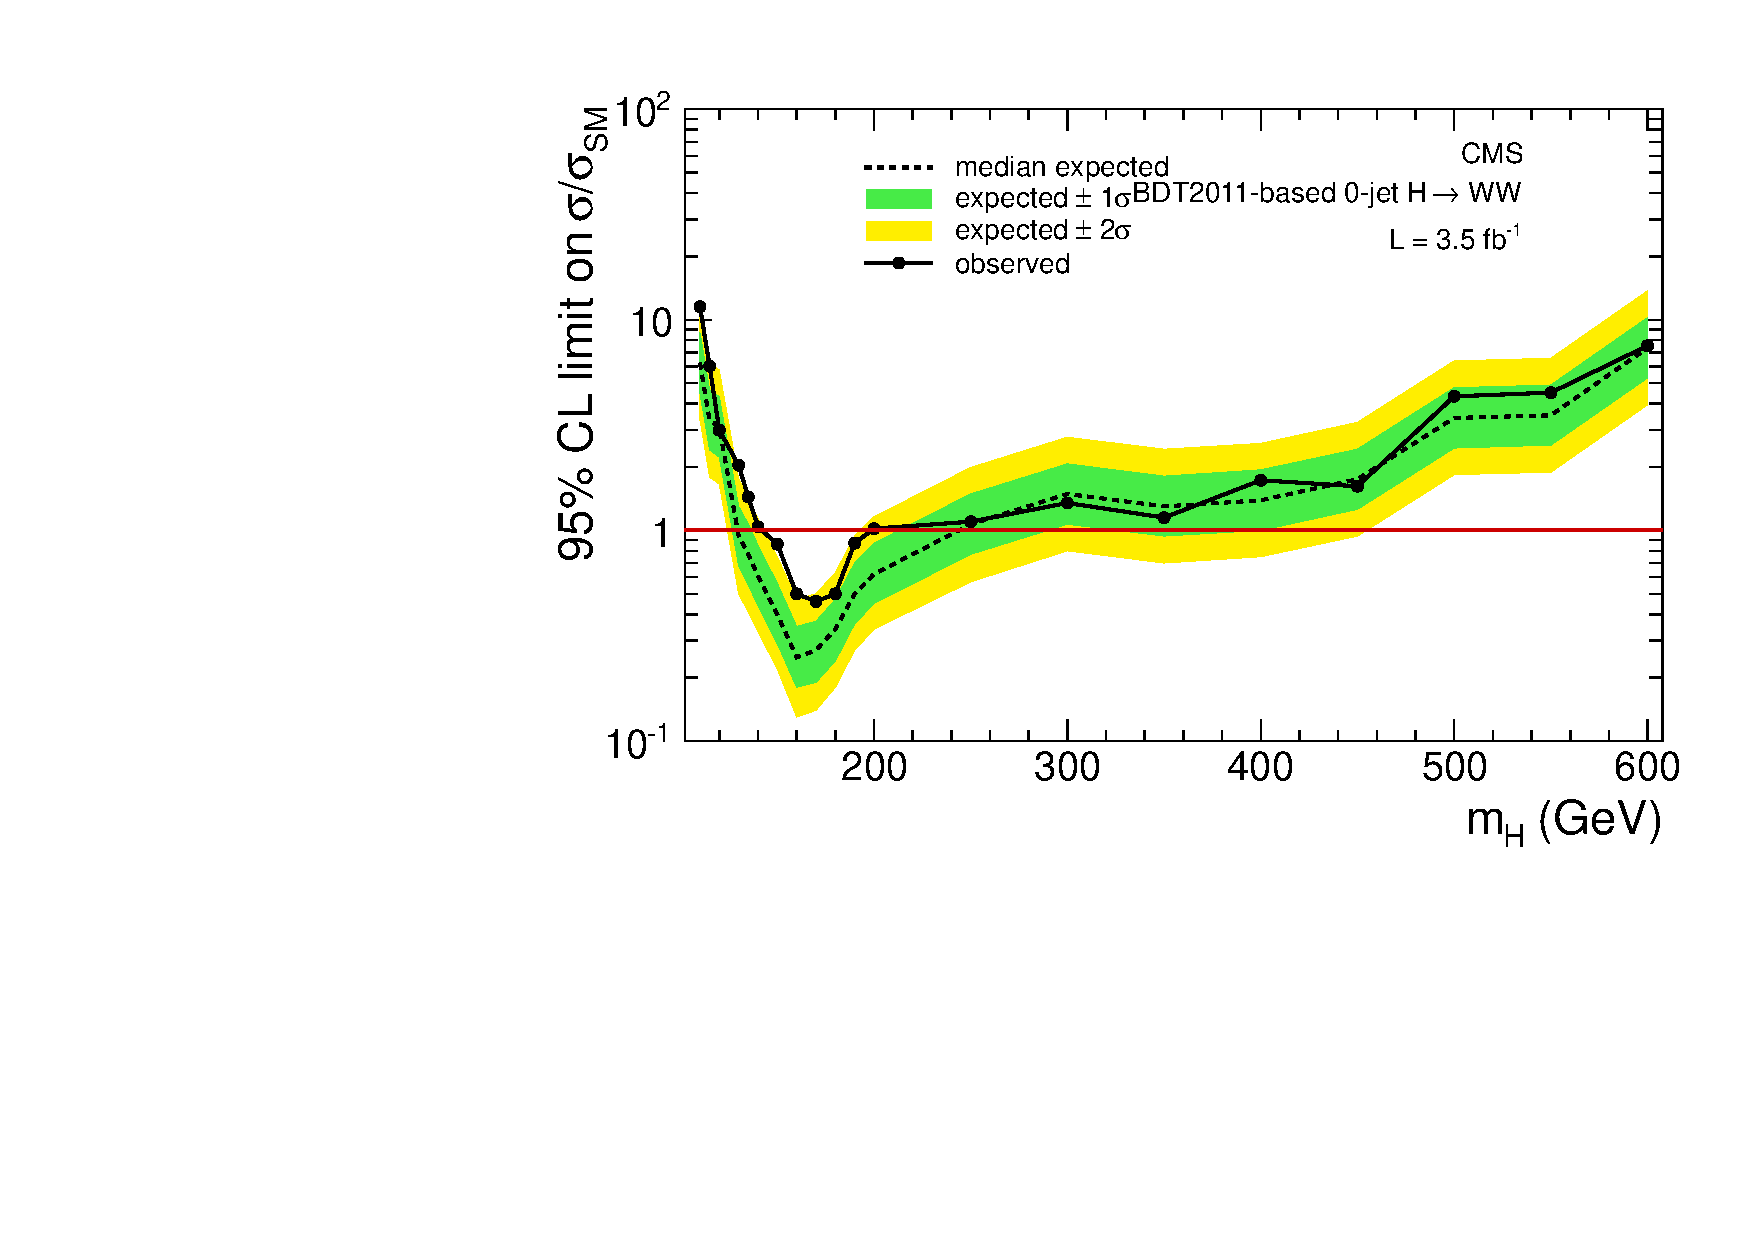
\includegraphics[width=.45\textwidth]{figures/limits_0j_BDT2011_shape_extended_8TeV.pdf}
}
\subfigure[shape-based zoomed 2011 BDT 0-jet bin]{
\centering
\label{subfig:sm_shape_zoom_BDT2011_0j}
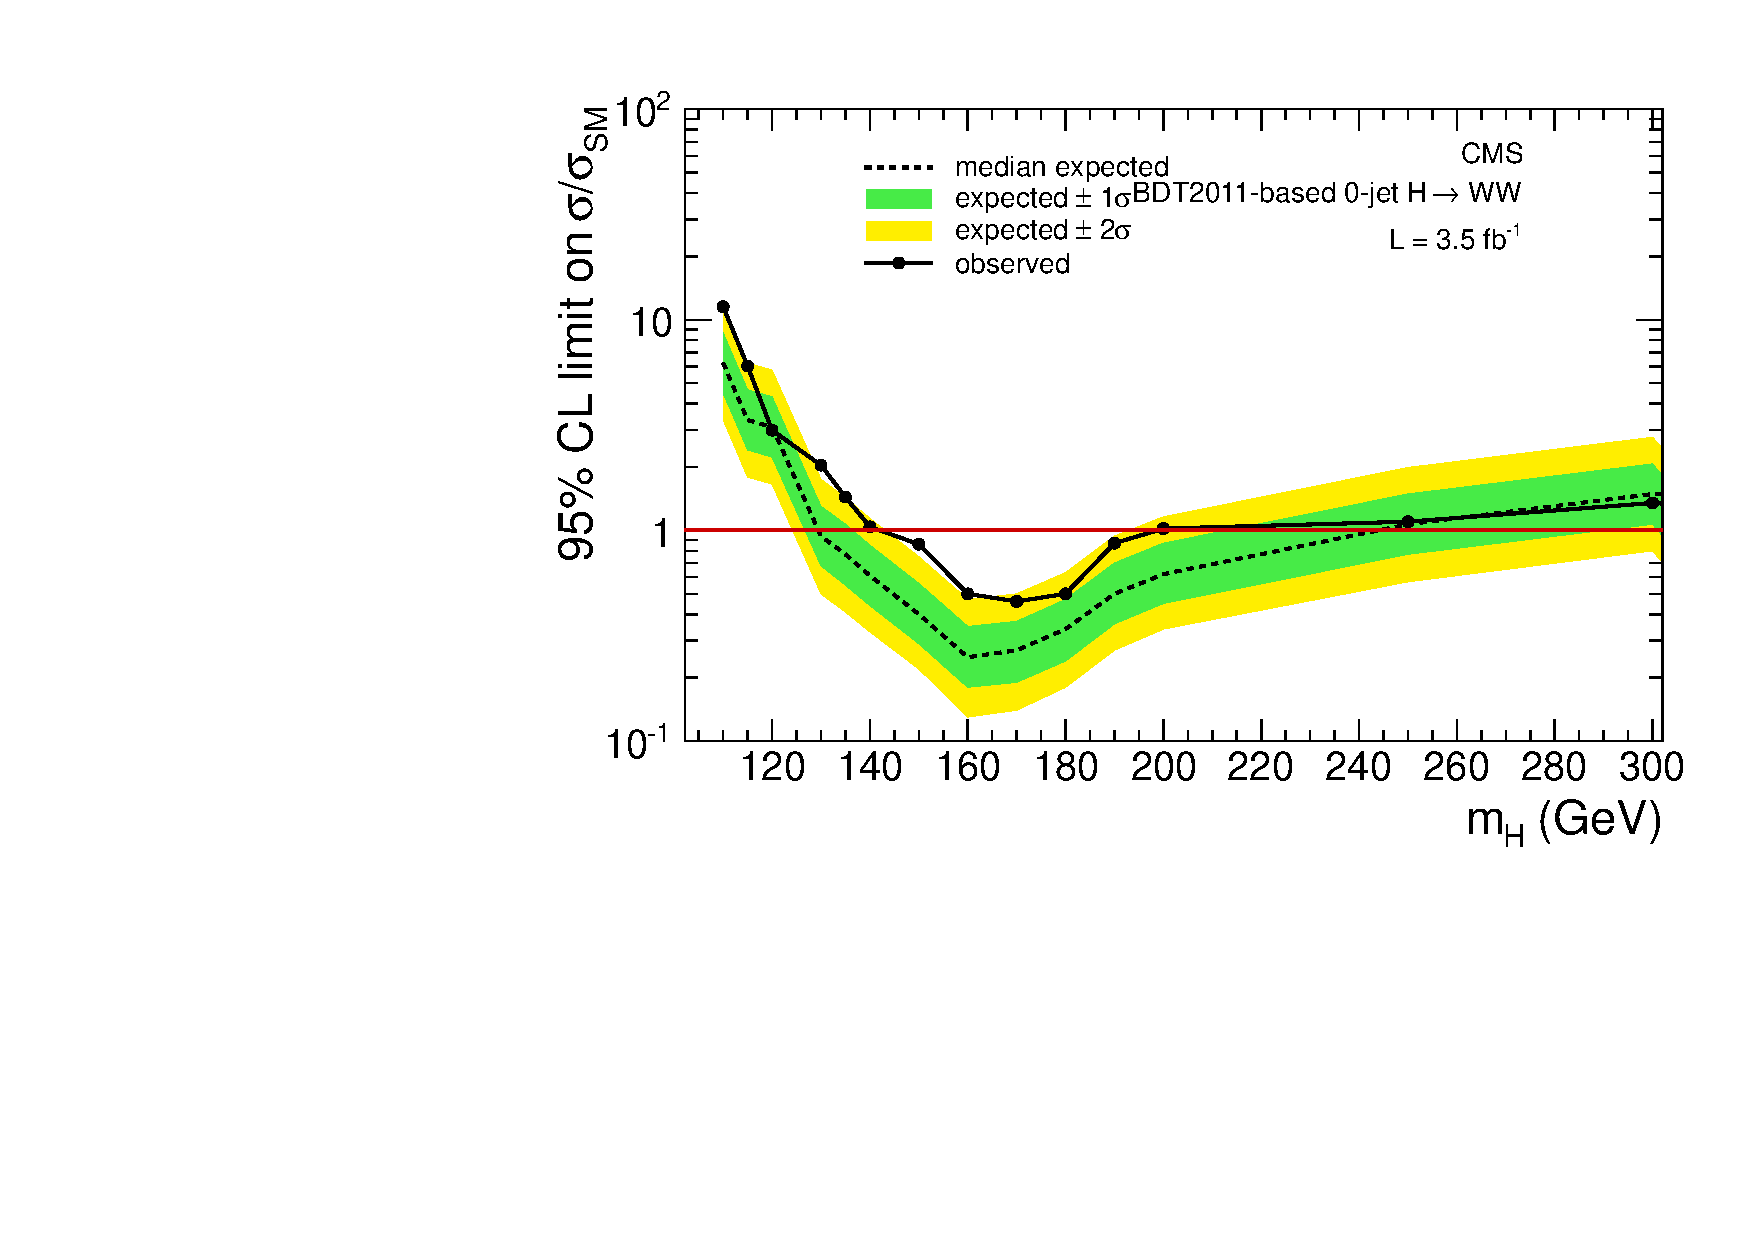
\includegraphics[width=.45\textwidth]{figures/limits_0j_BDT2011_shape_8TeV.pdf}
}
\centering
\subfigure[shape-based 2011 BDT 1-jet bin]{
\centering
\label{subfig:sm_shape_BDT2011_1j}
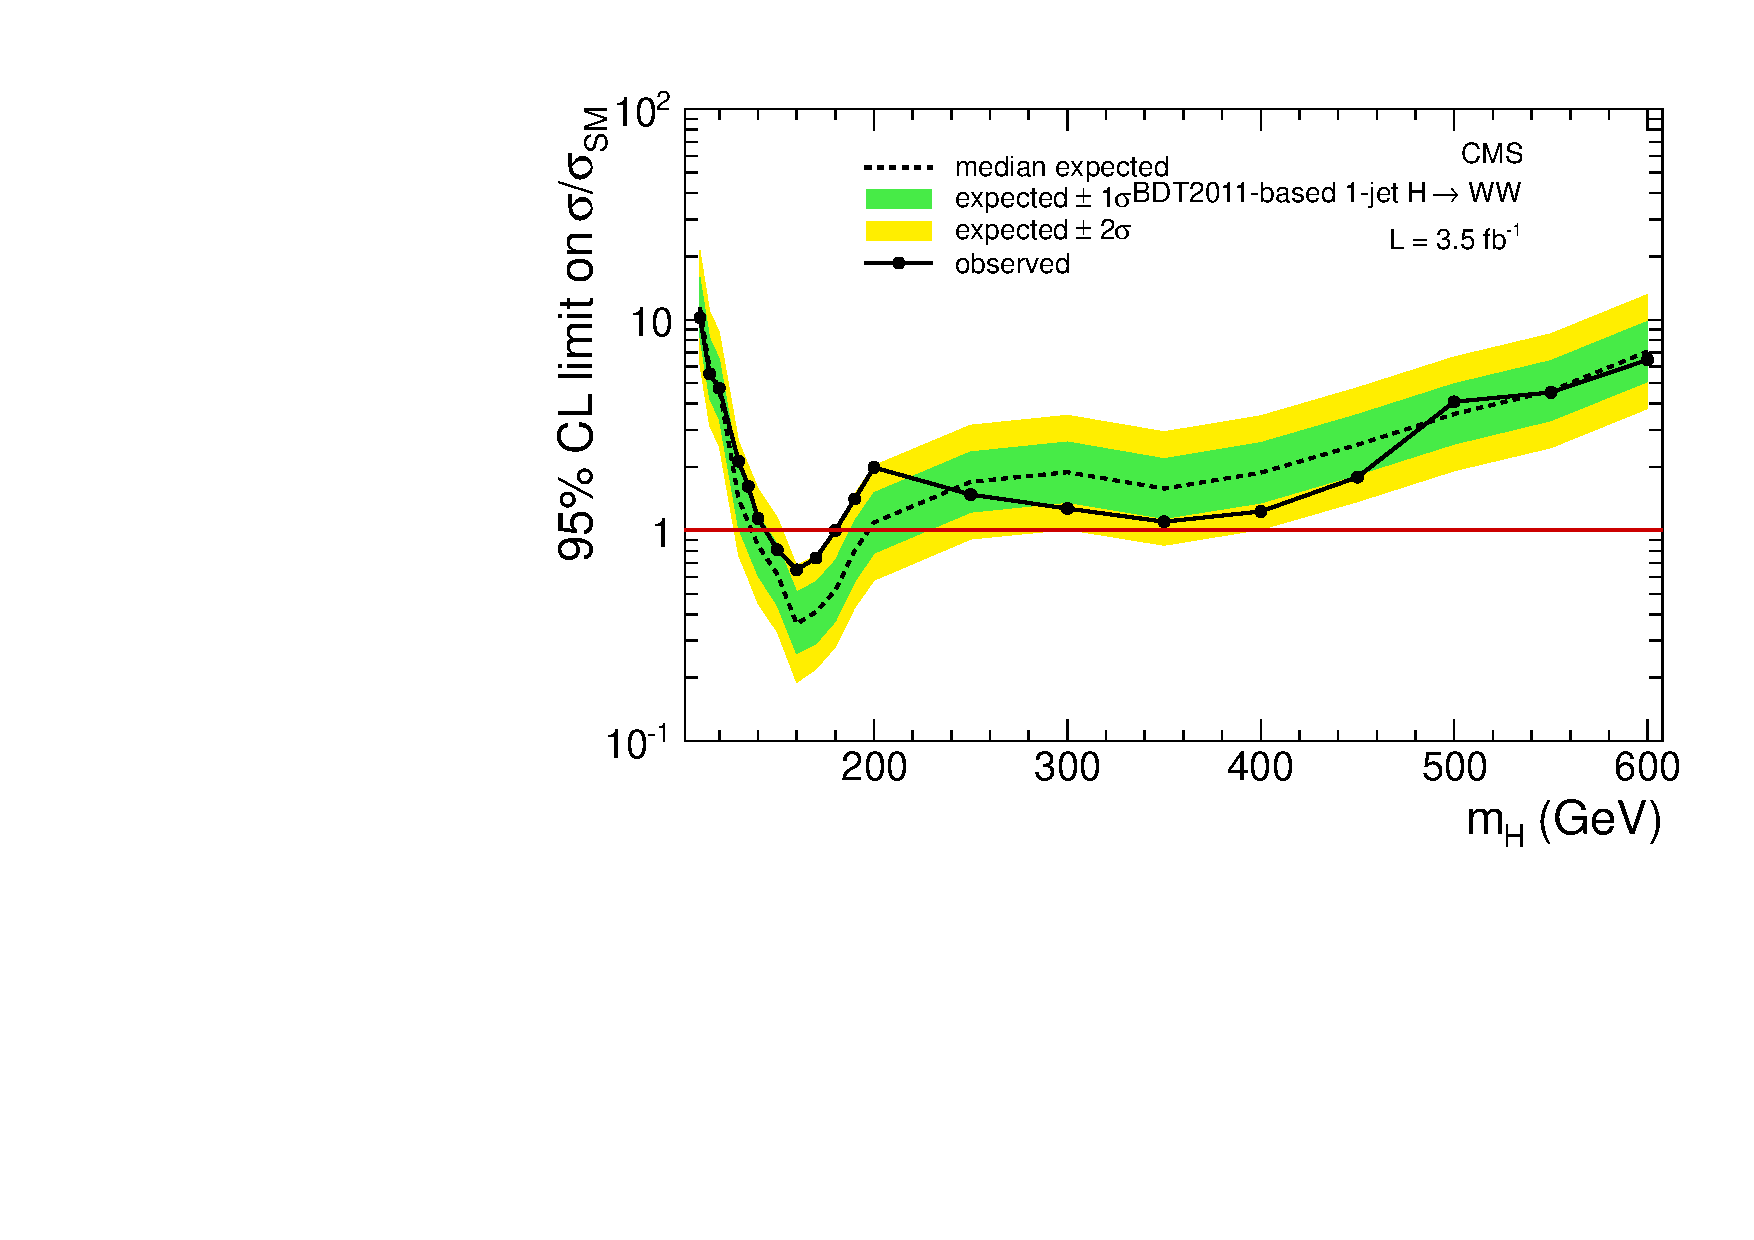
\includegraphics[width=.45\textwidth]{figures/limits_1j_BDT2011_shape_extended_8TeV.pdf}
}
\subfigure[shape-based zoomed 2011 BDT 1-jet bin]{
\centering
\label{subfig:sm_shape_zoom_BDT2011_1j}
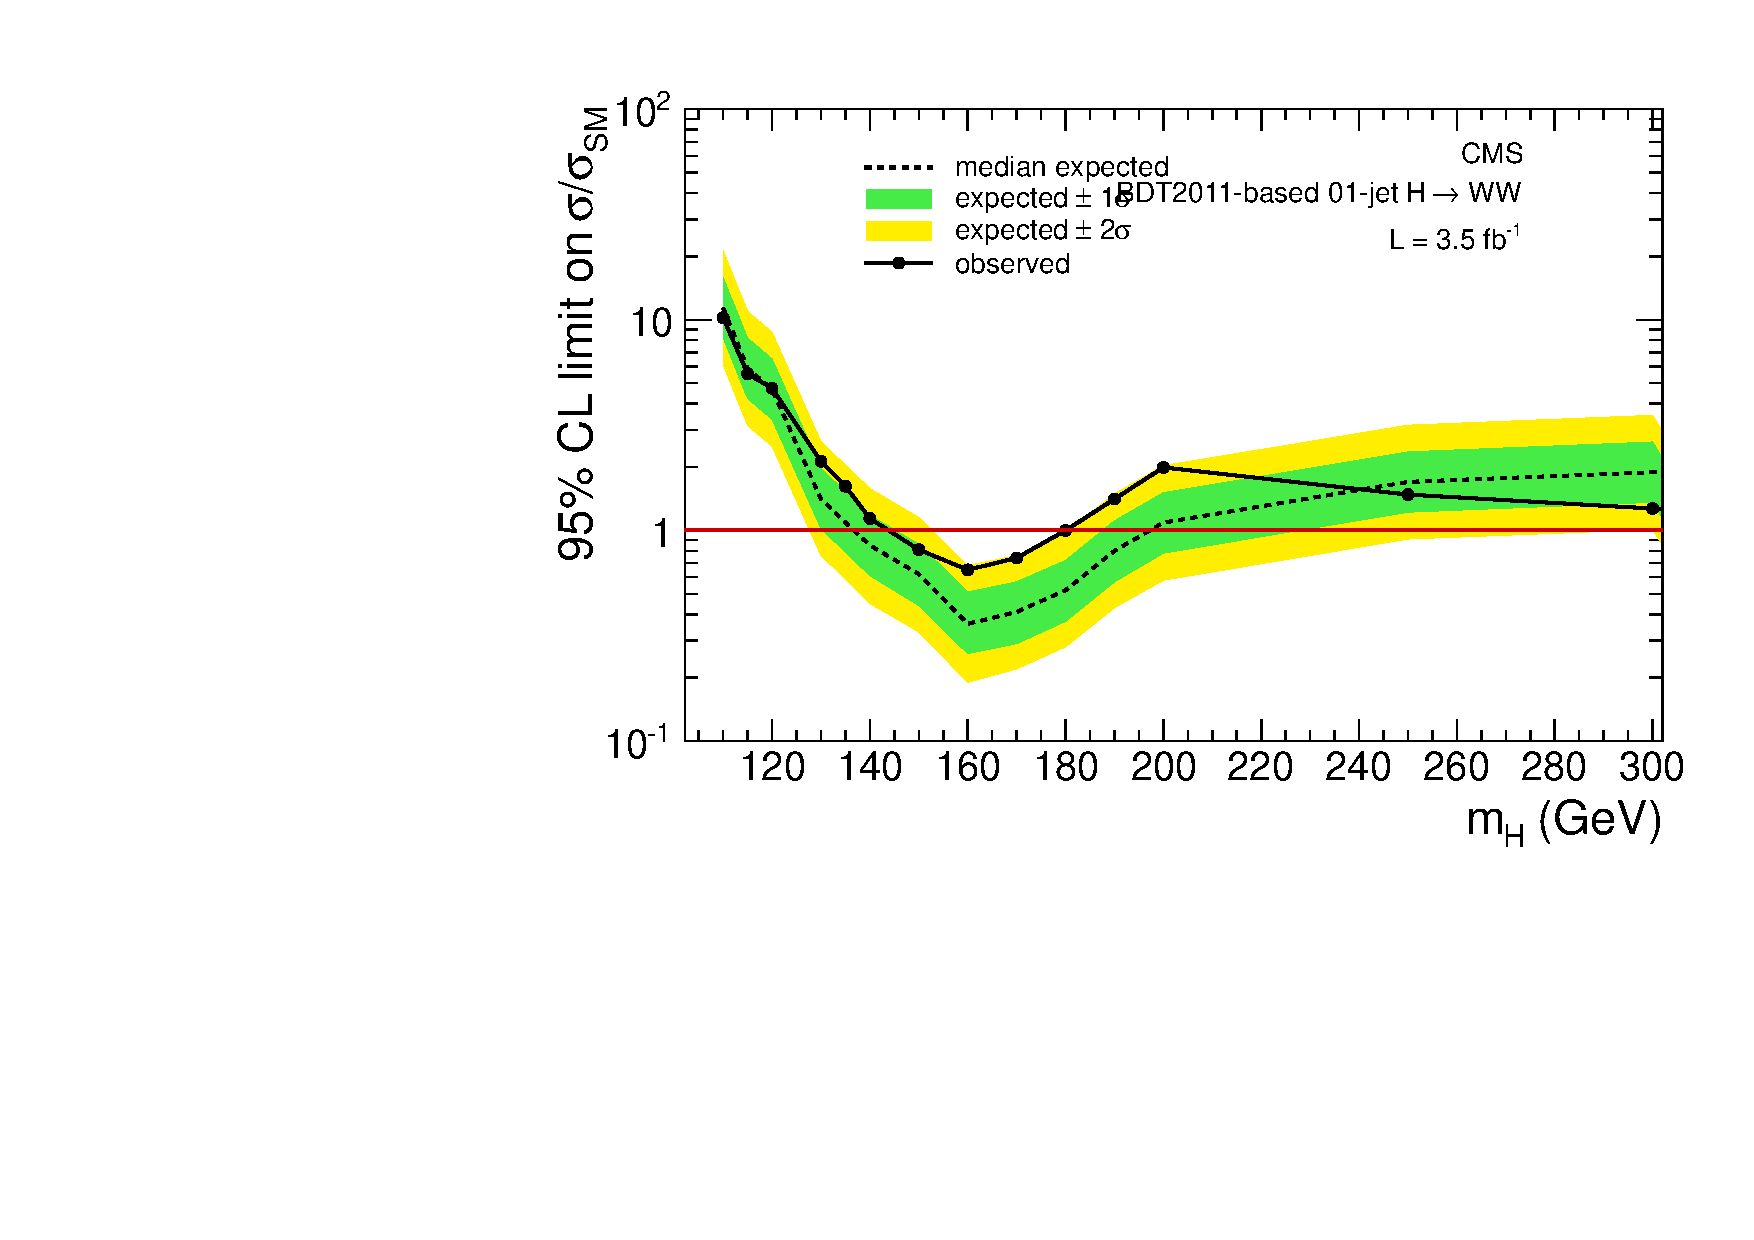
\includegraphics[width=.45\textwidth]{figures/limits_1j_BDT2011_shape_8TeV.pdf}
}
\centering
\subfigure[shape-based 2011 BDT 0/1-jet bins]{
\centering
\label{subfig:sm_shape_BDT2011_nj}
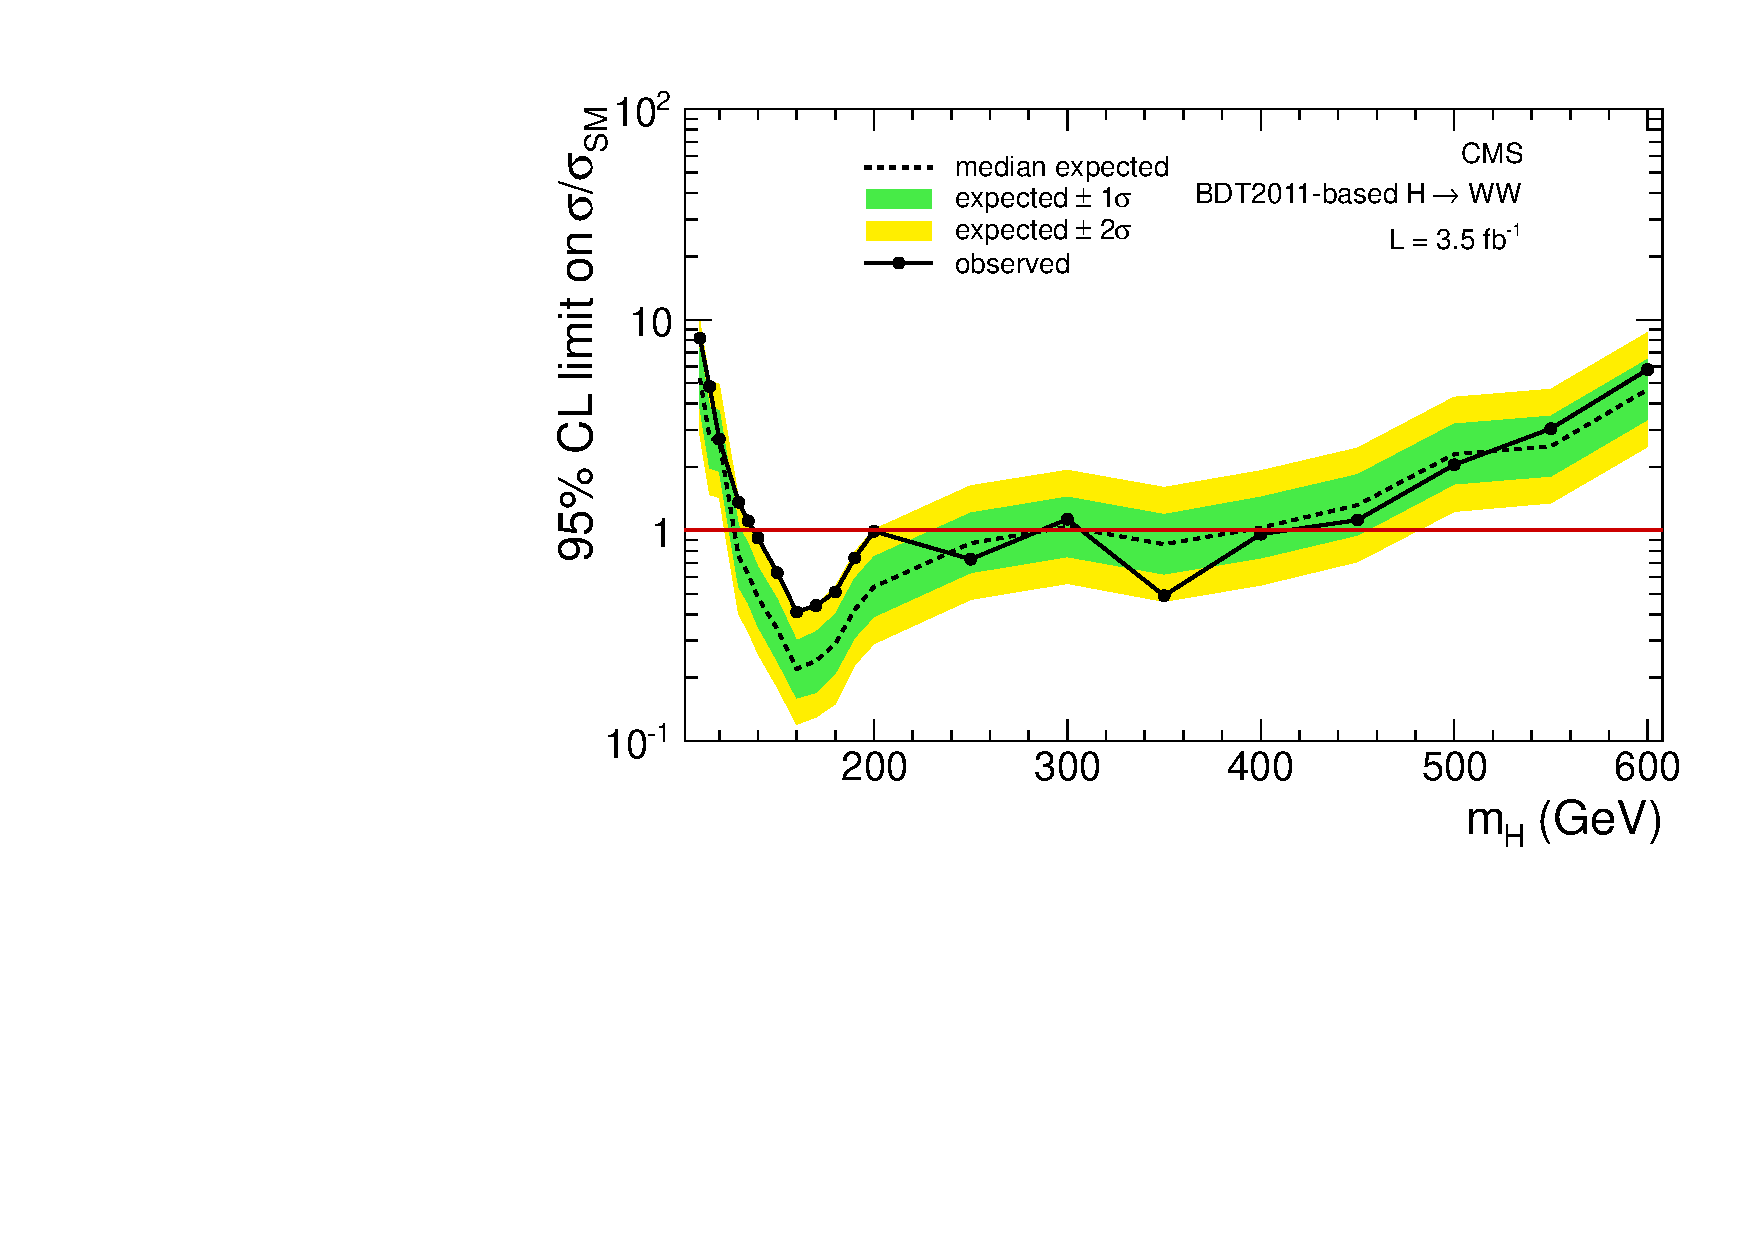
\includegraphics[width=.45\textwidth]{figures/limits_nj_BDT2011_shape_extended_8TeV.pdf}
}
\subfigure[shape-based zoomed 2011 BDT 0/1-jet bins]{
\centering
\label{subfig:sm_shape_zoom_BDT2011_nj}
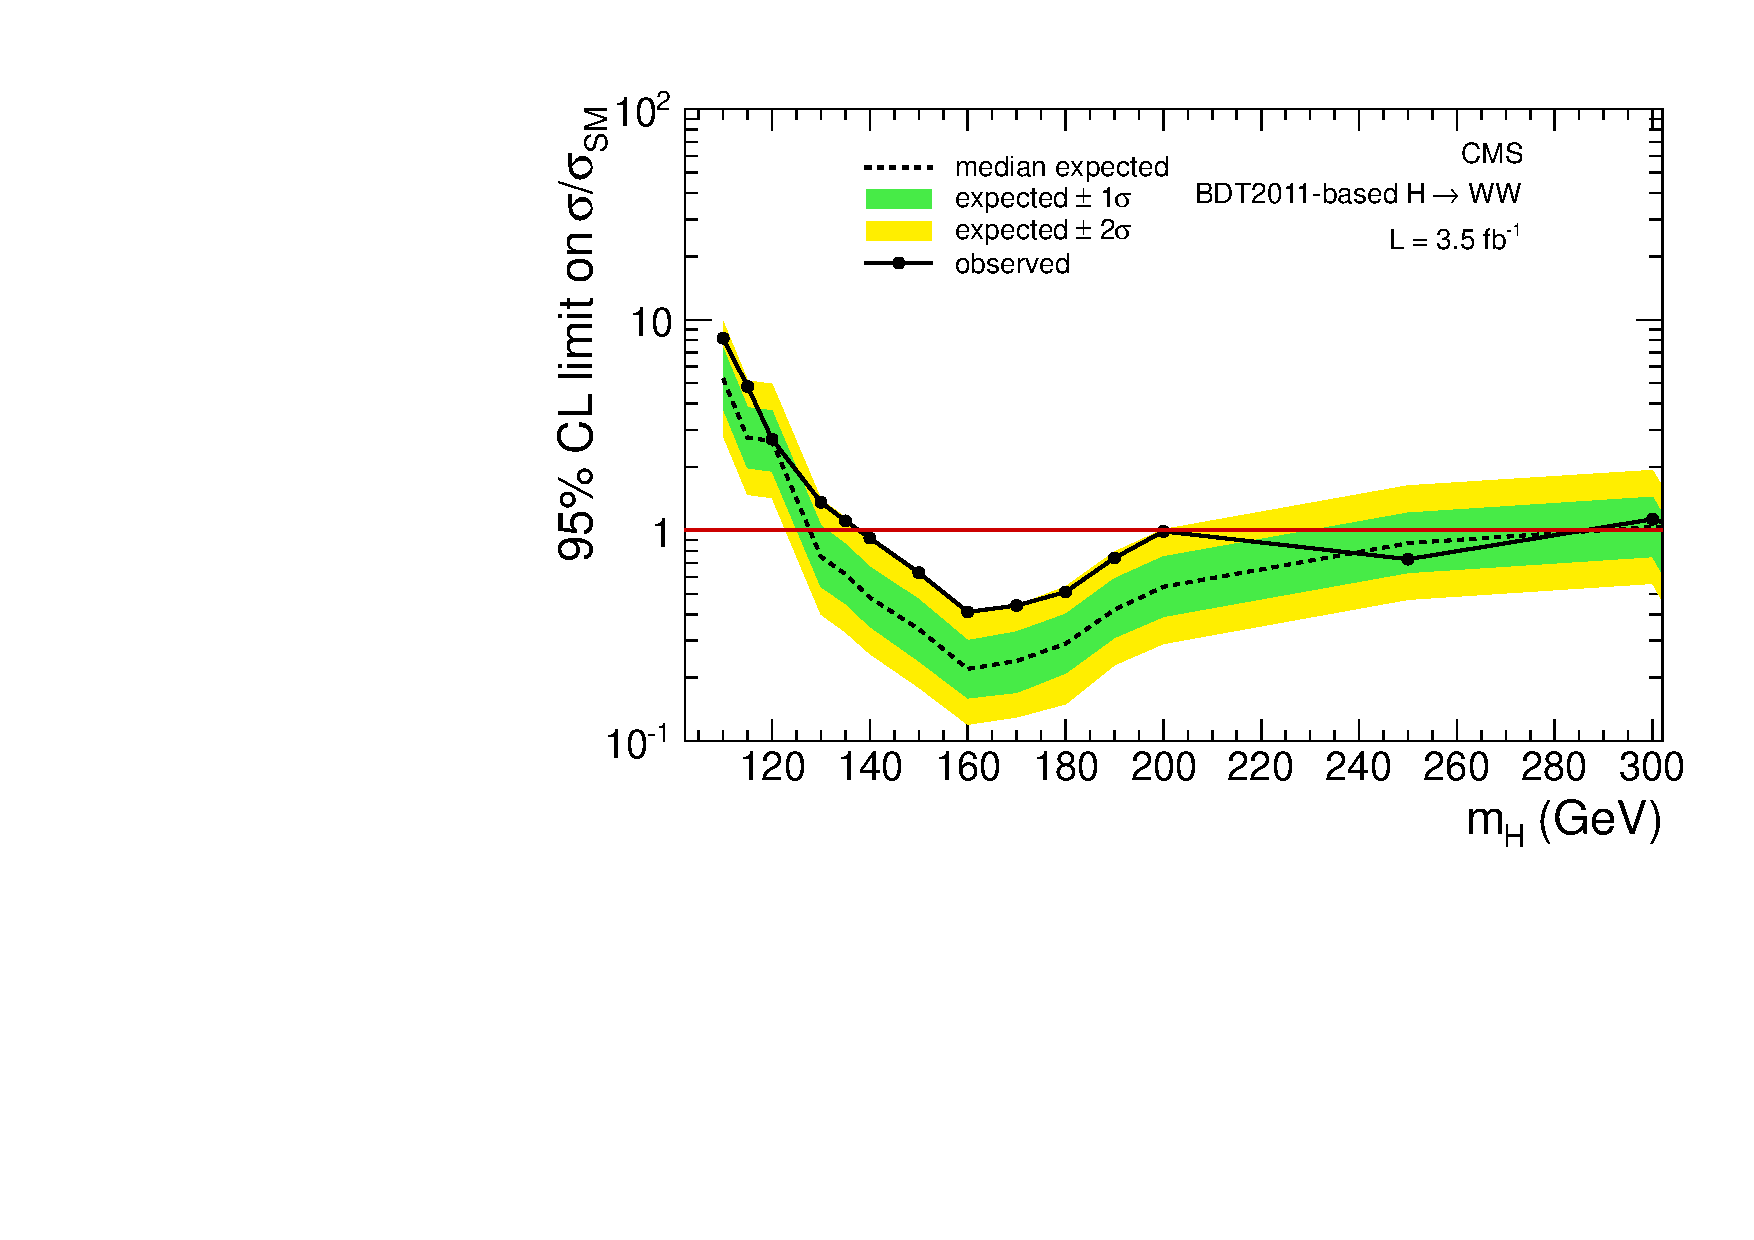
\includegraphics[width=.45\textwidth]{figures/limits_nj_BDT2011_shape_8TeV.pdf}
}
\caption{Expected and observed upper limits in the 0/1-jet bins for SM Higgs using the
  {\bf shape-based} 2011 BDT analysis with 3.5$\ifb$ of data.}
  \label{fig:uls_bdt2011}
\end{figure}
